
%(BEGIN_QUESTION)
% Copyright 2011, Tony R. Kuphaldt, released under the Creative Commons Attribution License (v 1.0)
% This means you may do almost anything with this work of mine, so long as you give me proper credit

This hand indicating controller (HIC-45) allows a human operator to position the control valve (HV-45) simply by pressing ``up'' and ``down'' buttons on the controller faceplate:

$$\includegraphics[width=15.5cm]{i02325x01.eps}$$

As the instrument technician, you need to configure the controller so that its digital display registers the valve stem's actual position: 0 on the controller display should represent 0\% open (fully shut) and 100 on the controller display should mean 100\% open.  This is necessary to make the interface easy to understand for the operators who must use it.  The challenge is, the valve is {\it air-to-close}, which means it requires {\it full} air pressure to close it all the way, and it opens wide at minimum pressure.

\vskip 10pt

There are two ways of accomplishing this goal.  The first way requires calibrating the I/P transducer to be reverse-acting (4 mA = 15 PSI ; 20 mA = 3 PSI).  The second way requires configuring the hand controller to be reverse {\it indicating} (4 mA = 100\% display ; 20 mA = 0\% display).  Suppose you chose the second method, where the I/P calibration is normal (e.g. 4 mA = 3 PSI) and the controller is {\it reverse-indicating} (e.g. 100\% display = 4 mA).  Given this controller configuration, complete the following table:

% No blank lines allowed between lines of an \halign structure!
% I use comments (%) instead, so that TeX doesn't choke.

$$\vbox{\offinterlineskip
\halign{\strut
\vrule \quad\hfil # \ \hfil & 
\vrule \quad\hfil # \ \hfil & 
\vrule \quad\hfil # \ \hfil & 
\vrule \quad\hfil # \ \hfil \vrule \cr
\noalign{\hrule}
%
% First row
{\bf Controller display} & {\bf Controller current} & {\bf I/P pressure} & {\bf Valve stem position} \cr
%
\noalign{\hrule}
%
% Another row
77.5\% &  &  &  \cr
%
\noalign{\hrule}
%
% Another row
 & 17.9 mA &  &  \cr
%
\noalign{\hrule}
%
% Another row
 &  & 4.29 PSI &  \cr
%
\noalign{\hrule}
%
% Another row
 &  &  & 64\% open \cr
%
\noalign{\hrule}
} % End of \halign 
}$$ % End of \vbox

\vskip 20pt \vbox{\hrule \hbox{\strut \vrule{} {\bf Suggestions for Socratic discussion} \vrule} \hrule}

\begin{itemize}
\item{} Explain why anyone would choose to use an air-to-close (fail open) control valve.
\item{} Explain why choosing to use a reverse-acting I/P might not be a good idea, considering fail-safe requirements of the system.
\item{} Write a linear equation in the form $y = mx + b$ to describe the current signal output from the controller ($y$) in terms of its displayed percentage ($x$).
\item{} Explain the distinction between a loop controller that is {\it reverse-acting} versus one that is merely {\it reverse-indicating}.
\item{} Explain the purpose of the diode in the circuit.
\end{itemize}

\underbar{file i02325}
%(END_QUESTION)





%(BEGIN_ANSWER)

$$\vbox{\offinterlineskip
\halign{\strut
\vrule \quad\hfil # \ \hfil & 
\vrule \quad\hfil # \ \hfil & 
\vrule \quad\hfil # \ \hfil & 
\vrule \quad\hfil # \ \hfil \vrule \cr
\noalign{\hrule}
%
% First row
{\bf Controller display} & {\bf Controller current} & {\bf I/P pressure} & {\bf Valve stem position} \cr
%
\noalign{\hrule}
%
% Another row
77.5\% & 7.6 mA & 5.7 PSI & 77.5\% open \cr
%
\noalign{\hrule}
%
% Another row
13.1\% & 17.9 mA & 13.43 PSI & 13.1\% open \cr
%
\noalign{\hrule}
%
% Another row
89.3\% & 5.72 mA & 4.29 PSI & 89.3\% open \cr
%
\noalign{\hrule}
%
% Another row
64\% & 9.76 mA & 7.32 PSI & 64\% open \cr
%
\noalign{\hrule}
} % End of \halign 
}$$ % End of \vbox

%(END_ANSWER)





%(BEGIN_NOTES)

Formula relating controller output display to current value:

$$y = \left(-16x \over 100 \right) + 20$$

\noindent
Where,

$y$ = Controller output current (mA)

$x$ = Controller display (0 to 100)

\vskip 10pt

The relationship between current and I/P output pressure, of course, is a simple and direct matter of converting 4-20 mA into 3-15 PSI.

\vskip 10pt

The valve's actual position, of course, should precisely match the controller's output display.










\filbreak \vskip 20pt \vbox{\hrule \hbox{\strut \vrule{} {\bf Virtual Troubleshooting} \vrule} \hrule}

\noindent
{\bf Predicting the effect of a given fault:} present each of the following faults to the students, one at a time, having them comment on all the effects each fault would produce.

\begin{itemize}
\item{} 
\item{} 
\item{} 
\end{itemize}


\vskip 10pt


\noindent
{\bf Identifying possible/impossible faults:} present symptoms to the students and then have them determine whether or not a series of suggested faults could account for all the symptoms, explaining {\it why} or {\it why not} for each proposed fault:

\begin{itemize}
\item{} 
\item{} 
\item{} 
\end{itemize}


\vskip 10pt


\noindent
{\bf Determining the utility of given diagnostic tests:} imagine the diode fails open in this system.  Present the operator's observation(s) to the students and then propose the following diagnostic tests one by one.  Students rate the value of each test, determining whether or not it would give useful information (i.e. tell us something we don't already know).  Students determine what different results for each test would indicate about the fault, if anything:

\begin{itemize}
\item{} {\it Valve remains 100\% open, regardless of controller output indication percentage}
\item{} Measure current at controller output -- {\bf Yes}
\item{} Measure current in parallel with diode -- {\bf Yes}
\item{} Measure current at I/P input -- {\bf Yes}
\item{} Measure voltage at I/P input -- {\bf Yes}
\item{} Check packing nut torque on control valve -- {\bf Probably no}
\item{} Crack fitting at I/P output port -- {\bf Yes}
\item{} Crack fitting at I/P supply port -- {\bf Yes}
\item{} Crack fitting at valve diaphragm port -- {\bf Yes}
\item{} Measure AC voltage at power terminals of controller -- {\bf No}
\item{} Measure $V_{34-35}$ -- {\bf Yes}
\item{} Measure $V_{13-14}$ -- {\bf Yes}
\item{} Measure $V_{12-13}$ -- {\bf Yes}
\item{} Measure $V_{14-15}$ -- {\bf Yes}
\end{itemize}


\vskip 10pt


\noindent
{\bf Diagnosing a fault based on given symptoms:} imagine the ??? fails ??? in this system (but don't tell this to students!).  Present the operator's observation(s) to the students, have them consider possible faults and diagnostic strategies, and then tell them the results of tests they propose based on the following symptoms, until they have properly identified the nature and location of the fault:

\begin{itemize}
\item{} {\it }
\item{} 
\item{} 
\end{itemize}

%INDEX% Basics, control: direct versus reverse controller output indication
%INDEX% Control, basics: direct versus reverse controller output indication

%(END_NOTES)


